\documentclass[linenumbers, ]{aastex631}

\newcommand{\vdag}{(v)^\dagger}
\newcommand\aastex{AAS\TeX}
\newcommand\latex{La\TeX}

\usepackage{amsmath}
%\usepackage{graphicx}
\usepackage{subfig}

\journalinfo{}

\begin{document}

\title{Tracking Mass Transfer between M31 and the Milky Way using Galactic Simulation Data}

%% REFS FOR IMAGES 1 and 4 not working. I don't understand why, and nothing I tried would fix it.


\author{Avichal Kaul}
\affiliation{Steward Observatory, University of Arizona, 933 N. Cherry Ave, Tucson, AZ 85721, USA}

\begin{abstract}
Galactic Mergers are a process during which two or more galaxies fall together to form one galaxy. The structure of the galaxy undergoes massive changes, which can have huge consequences for stellar formation and galactic evolution. Our aim was to study the nature of the mass transfer during the merger between M31 and the MW. This will help further our understanding of galactic evolution, and help explain where mass transferred between the galaxies ends up. We find that almost no material ends up gravitationally unbound. We also find that most mass transfer between the galaxies results in mass concentrated around the galactic centres. This tells us that the effects of dynamical friction are immense, and effectively trap any particles within the combined system's gravitational well. The particles that are transferred often end up near the galactic centre, though particles that are flung outward and then fall inwards might join them in the more homogeneous irregular galaxy that results from this merger.
\end{abstract}

\keywords{Stellar Disk -- Stellar Bulge -- Major Merger -- Dynamical Friction  -- Tidal Tails}

\section{Introduction}

A galaxy is a gravitationally bound collection of stars whose properties
cannot be explained by a combination of baryons and Newton’s laws of gravity \citep{Willman_Strader_2012}. It consists, broadly, of the Bulge - a tightly-packed group of stars surrounding the galactic centre \citep{Minniti_2007}, the Disk - a thin, circular collection of stars and gas, and the Dark Matter Halo - an object whose presence is inferred from its effect on the rotation curve of the Disk and the Bulge, as we cannot observe it directly.

Galactic Mergers are a process during which two or more galaxies, due to a combination of gravitational attraction and dynamic friction, fall together and merge into one galaxy. During this process, the star formation rate is increased hugely \citep{Moster_2011} and the structure of the galaxy undergoes massive changes. An example of one of these mergers can be seen in Figure 1.

Galactic mergers are an incredibly important aspect of galactic evolution. \citep{1978MNRAS.183..341W} notes that the $\lambda\text{CDM}$ model of cosmology suggests present day galaxies are formed from successive accretions and mergers of smaller entities. These successive accretions and mergers have been linked to star formation \citep{Barnes_2004} due to the sudden collision and compression of large HI clouds. Even the formation of tidal tails, an elongated region of gas and stars that extends from a galaxy, are directly linked to the tidal forces exerted by other galaxies.

Mass transfer during mergers is very common, along with galactic material being flung out to immense distances. Some of the most famous examples of these are the Mice galaxies, modelled in \citep{Privon_2013}, which are a prime example of this transfer. Figure 1 shows us how a galactic merger can disrupt the structure of the galaxy, and how the transferred material is likely to evolve. 

While the process of galaxies accreting and merging is well understood, there are still various open questions in this field. For instance, the role that supermassive black holes and Active Galactic Nuclei have to play during a merger \citep{Silverman_2011}. In fact, we still cannot explain bulge formation as a function of galactic mergers \citep{Brooks2016}, which is a huge gap in our scientific understanding.

\begin{figure}
    \centering
    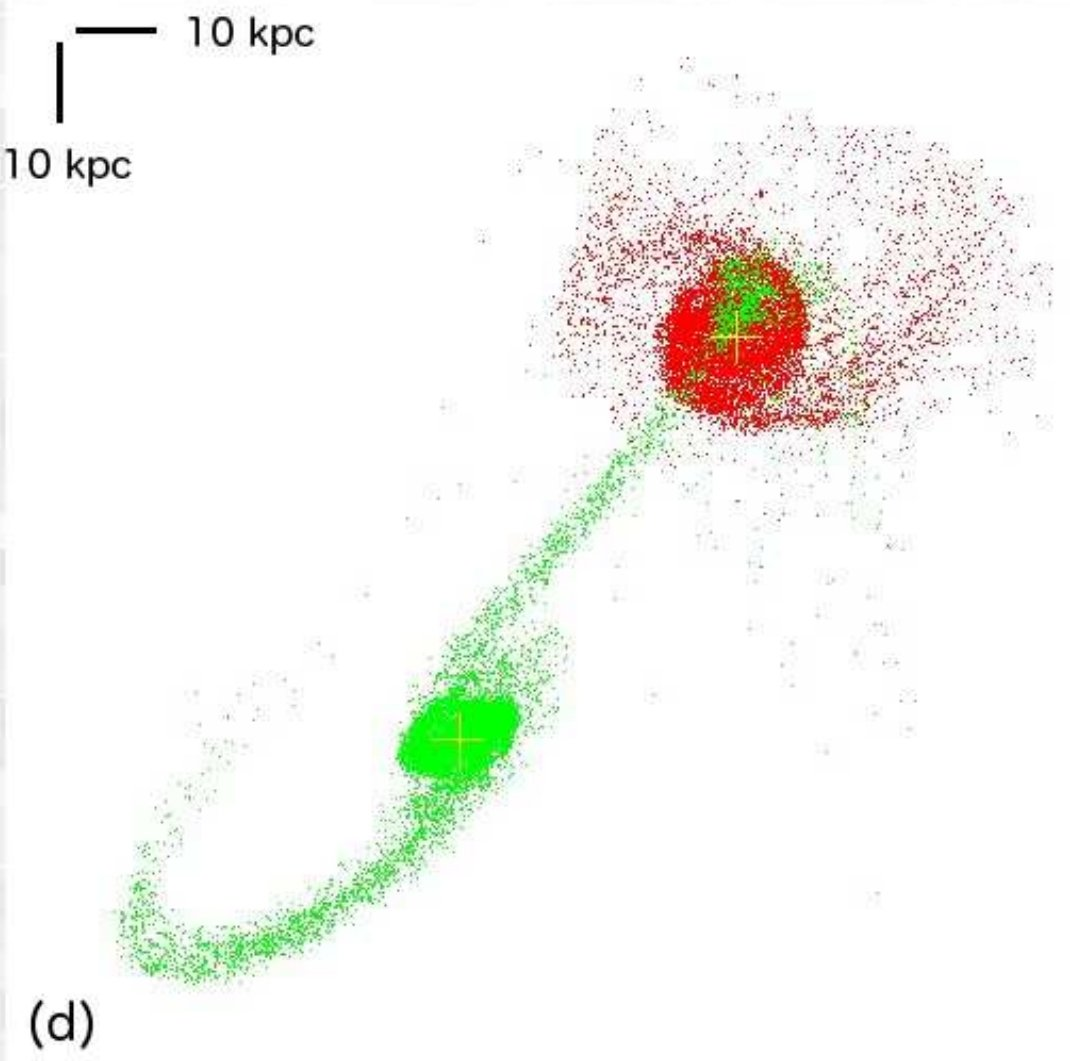
\includegraphics[width = 0.5\linewidth]{page08_1.jpg}
    \label{fig:Privonimage}
    \caption{A snapshot from a galactic merger simulation that shows mass transfer between two galaxies. Figure from \citep{Privon_2013}.}
\end{figure}


\section{This Project}

In this paper, we will study the evolution of the Milky Way/M31 galactic merger. Specifically, the nature of the mass transfer during the merger and the evolution of the system with time. We will track statistics such as the total energy of each particle with time, the mean and standard deviations of the results, and the distribution of the velocities of the particles.

This question hopes to address, or at least provide some insight into, how bulge formation relates to galactic mergers. We can, over the course of the merger, check on the structure of the bulge and how it varies with time. 

This is important not just for galactic evolution, but for stellar evolution as well. Stellar formation skyrockets during a galactic merger, and it is in the best interest of all astronomers that we know its causes.

In the following sections, we will consider Galaxy A (stationary in its reference frame) and Galaxy B (colliding with Galaxy A). In actuality, both galaxies are moving towards each other. All the analysis described here will be performed on both the galaxies separately.

\section{Methodology}

% replace time range w/ the actual time in Gyr
Gravitational N-body simulations are numerical simulations of the equations of motion for N particles interacting gravitationally \citep{trenti2008gravitational}. We are using N-body galactic simulations from \citep{Besla}, which provides us with a full simulation of the MW colliding with M31 over a time range of multiple Gyr. 

We wish to characterise the mass transfer at different points in the merger process. Especially of interest are the timesteps right after a close encounter, as a lot of material will be transferred between the galaxies at this time and will gradually settle into place. It will be interesting to see what material gets assimilated into another galaxy, and what material becomes gravitationally unbound. An example of what this looks like can be seen in Figure 1, where you can see the mass transfer between colliding galaxies. This image shows what material has been transferred, but we will also be evaluating how strongly said material is gravitationally bound. 


To check whether or not particles are gravitationally bound, we need to compare their Kinetic Energy ($T$) to their Potential Energy ($\phi$), which are given below.

\begin{gather}
T = \frac{1}{2} mv^2 \\
\phi = -\frac{GM(R)}{R}
\end{gather}

Here, $m$ is the mass of the particle ($M_\odot$), $v$ is the velocity of the particle (km/s), $G$ is the Universal Gravitational Constant, $M(R)$ is the mass $M_\odot$ enclosed within galactocentric radius $R$ (kpc) of the galaxy. We will be using the Hernquist profile \citep{1990ApJ...356..359H} to find $M(R)$.

\begin{gather}
    \rho(r) = \frac{\rho}{(\frac{r}{r_s}(1+\frac{r}{r_s}^3))}\\
    M(R) = 4/3\pi\rho(r)r^3
\end{gather}

Where $r$ is the galactocentric radius (kpc) and $r_s$ is the scale radius of the Dark Matter Halo (kpc). This must be found computationally.

Our plots will show the location of all particles of each galaxy relative to one another projected onto a 2D representation. Some will show simple mass transfer between galaxies, while others will show which particles are gravitationally bound and which are not, and finally a representation of the velocity dispersion of particles. We can also make a 3D plot to properly discern which part of the galaxy matter has ended up in.

\subsection{Mass Transfer}

We can track the process of exchanging material by labelling the particles in the simulation with the name of their progenitor, then - after an encounter - checking to see if any particles have been exchanged between the galaxies. This only requires us to know the location of each particle, and the location of the galactic centre. For instance: we can use our previously developed code to find the location of Galaxy B's centre, and then check if any of the particles from Galaxy A have ended up there.

\subsection{Exchanged Material and its Kinematics}

To find which region of the galaxy the particles end up in, we can use a similar approach. As we know the position of the particles Galaxy A has exchanged with Galaxy B, we can check the main type of Galaxy B particle that surrounds them. Similarly, we can check if the particles rotate with the disk by calculating the velocity vector of Galaxy A's particles and comparing them to Galaxy B's particles. 

Finally, to track the total mass transfer over time, we can continue measuring how many particles have switched galaxies at regular timesteps until the galactic merger is complete.

\subsection{Evolution with Time}

I expect that, during the first couple of close encounters, most of the exchanged material will end up near the galactic centre. We can see this happening in simulation data (e.g. in Fig. \ref{fig:Privon image}. This makes sense, as the galactic centre is where most of the baryonic matter in the galaxy is concentrated. But, over time, the two galaxies will merge completely, so the material will all fall together into an elliptical galaxy.

\begin{figure}
    \centering
    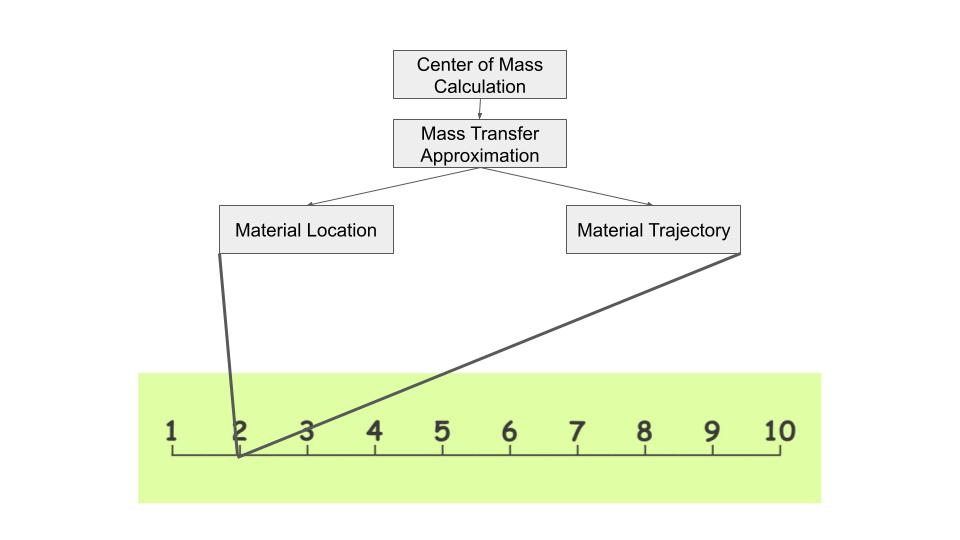
\includegraphics[width = \linewidth]{Untitled presentation.jpg}
    \label{fig:Untitled image}
    \caption{The proposed pipeline for data processing. At each simulation timestep (numbers 1-10 chosen for illustrative purposes), code is run to determine each property of the transferred material from top to bottom. This gives us an excellent idea of the evolution of the system with time.}
\end{figure}

\section{Results}

\begin{figure}[ht!]
\centering
   \subfloat[\label{genworkflow}]{%
      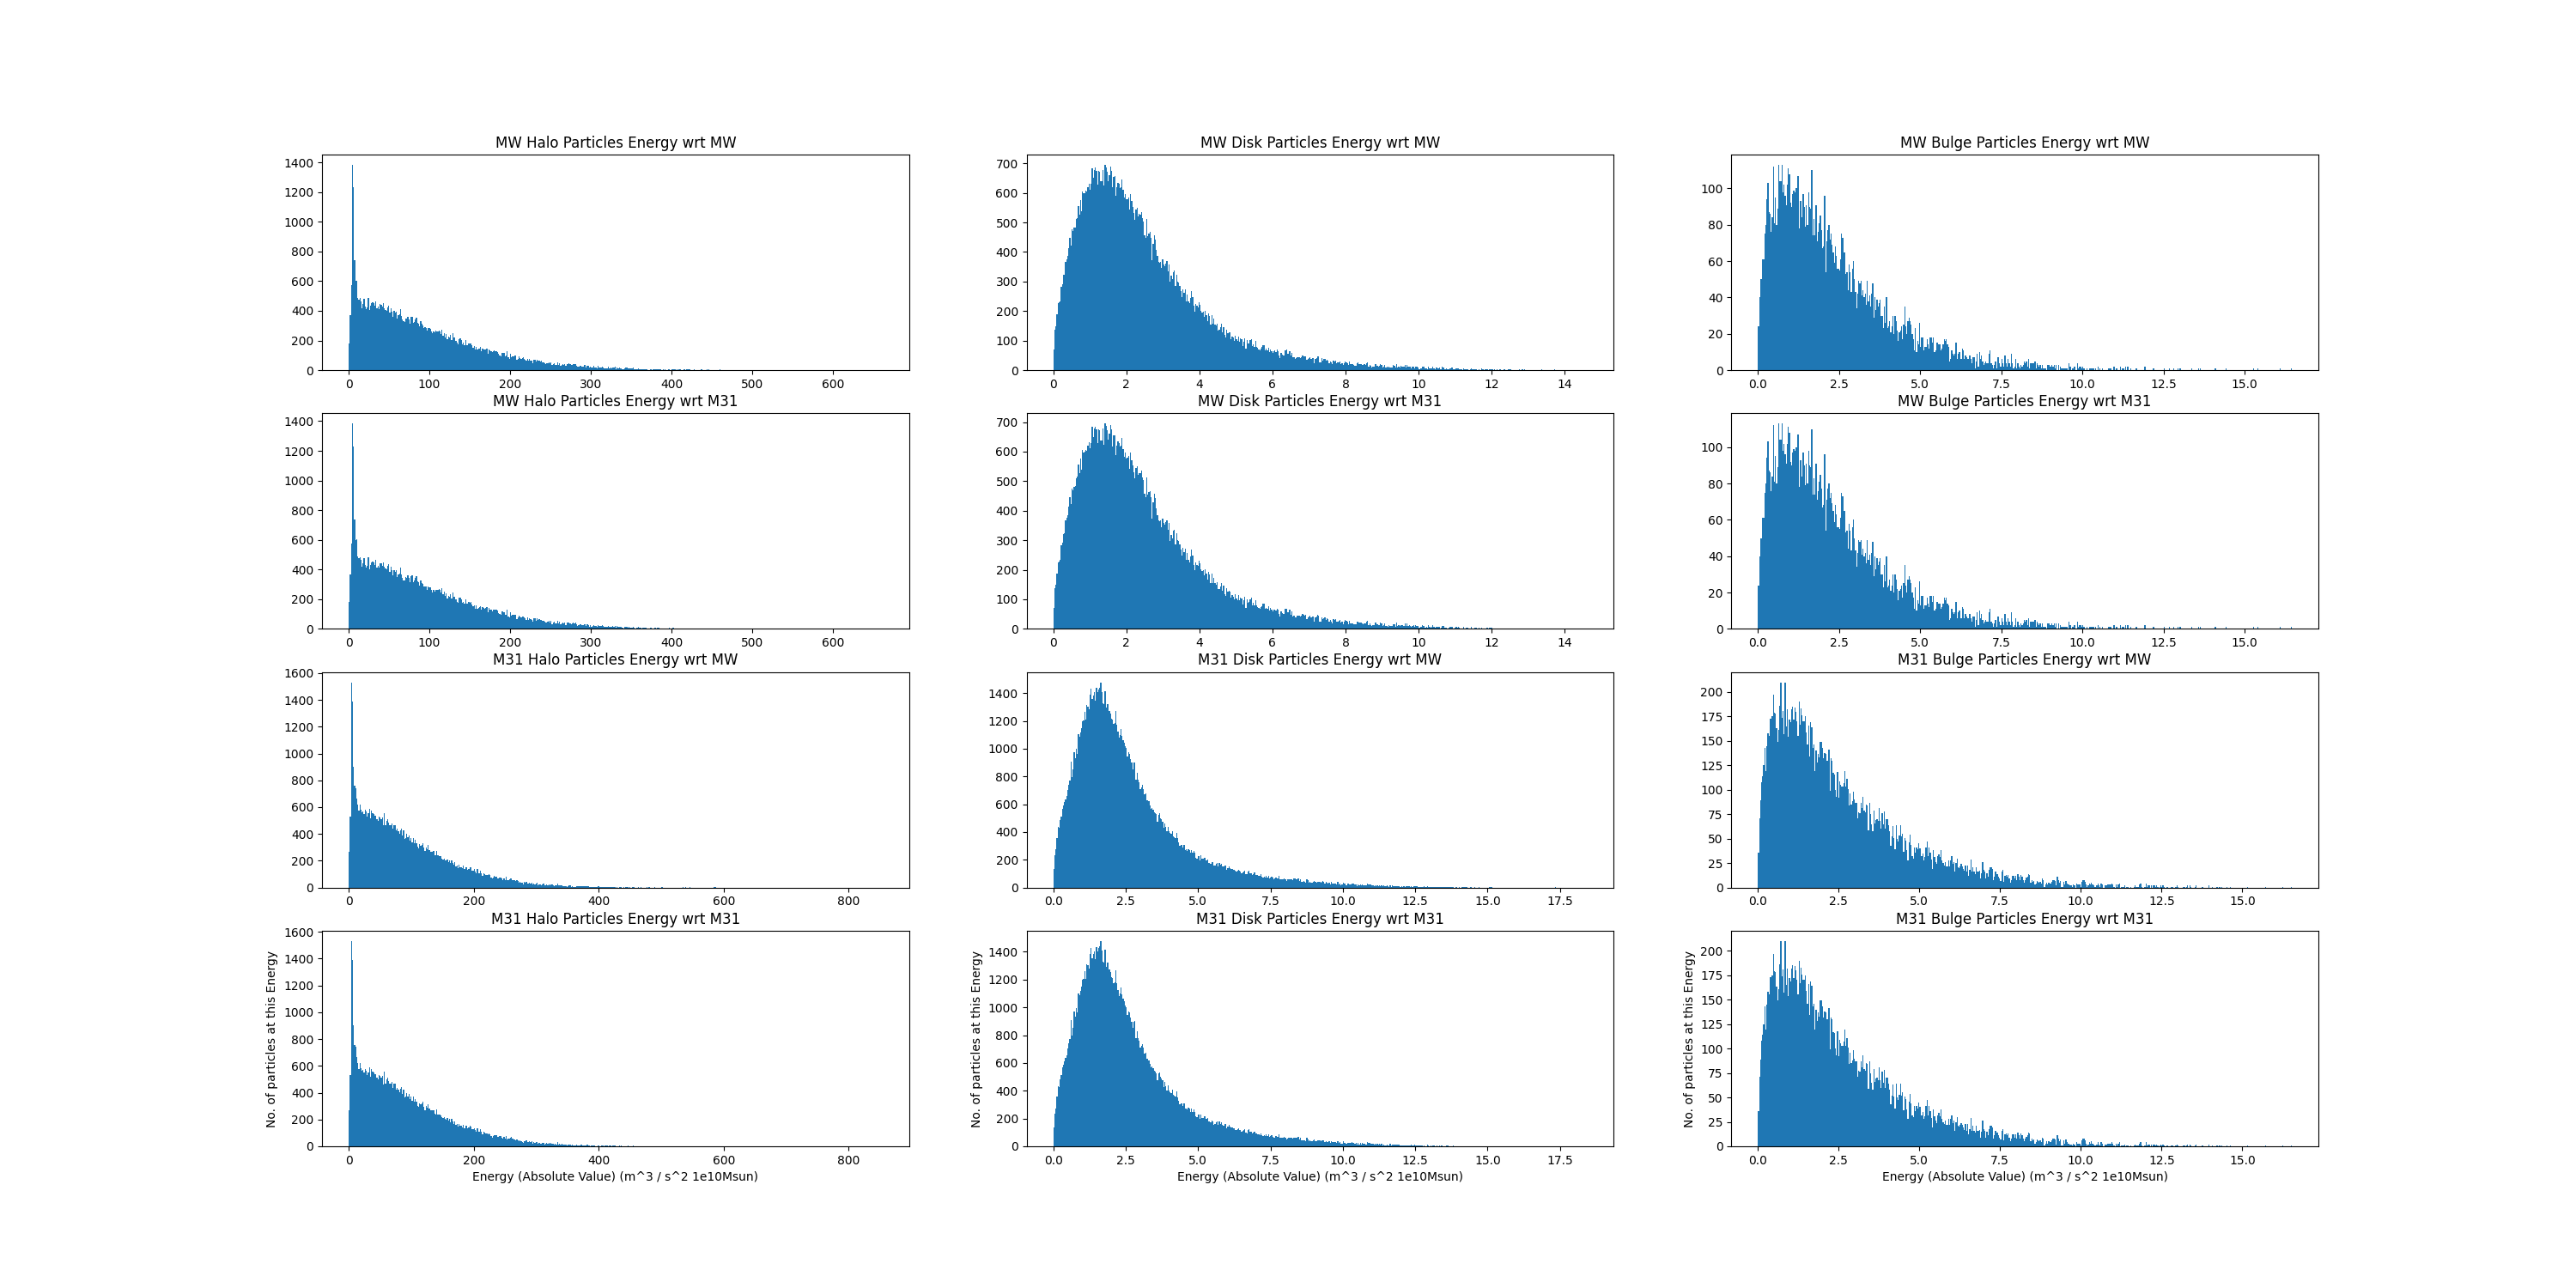
\includegraphics[trim=20 40 50 30,clip, width=0.8\textwidth]{figures/350.png}}
      
   \subfloat[\label{pyramidprocess} ]{%
      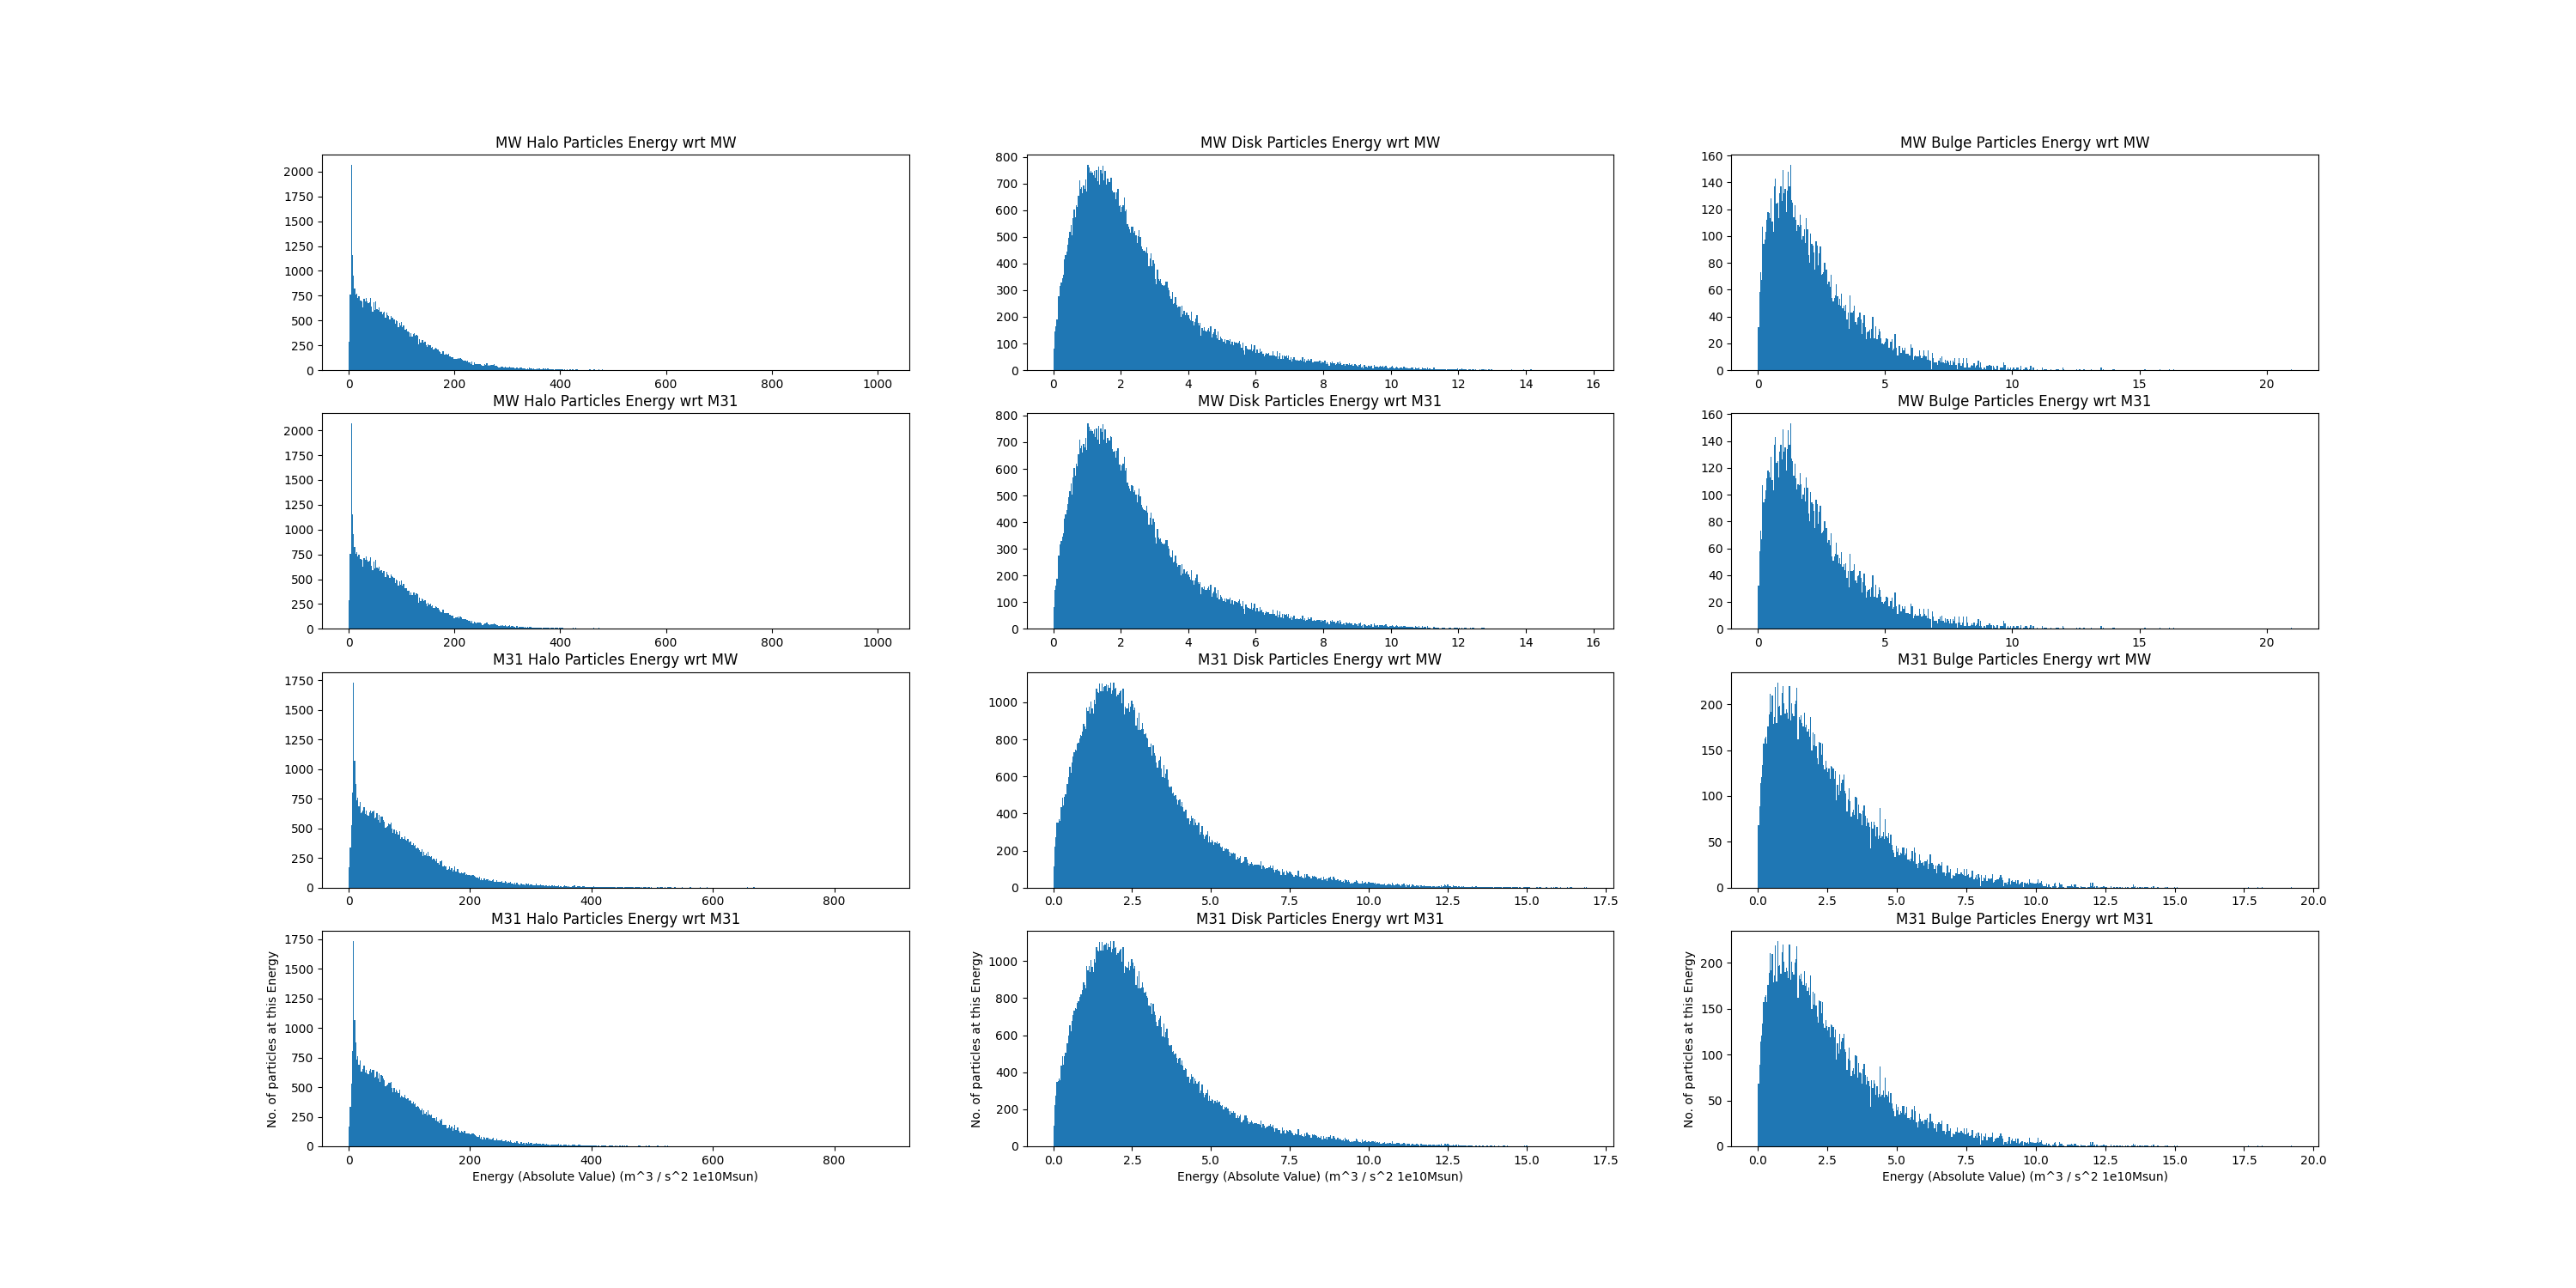
\includegraphics[trim=10 40 10 30,clip, width=0.8\textwidth]{figures/400.png}}
      
\caption{\label{fig:potentialdists} Histograms of energy distributions ($M_\odot km^2/s^2$) pre- and post- first close encounter. The different particle types are Halo, Disk, and Bulge, from left to right. From top to bottom: the total energy for a particle in the MW wrt the MW, the total energy for a particle in the MW wrt M31, the total energy for a particle in M31 wrt the MW, and the total energy for a particle in M31 wrt M31. (a) Snapshot 350; (b) Snapshot 400. We do not see much difference, even though the galaxies are tearing themselves apart. This tells us that the Potential terms (a) vastly exceed the Kinetic Energy terms, and (b) that most particles will remain gravitationally bound to the system.}
\end{figure}


\begin{figure}
    \centering
    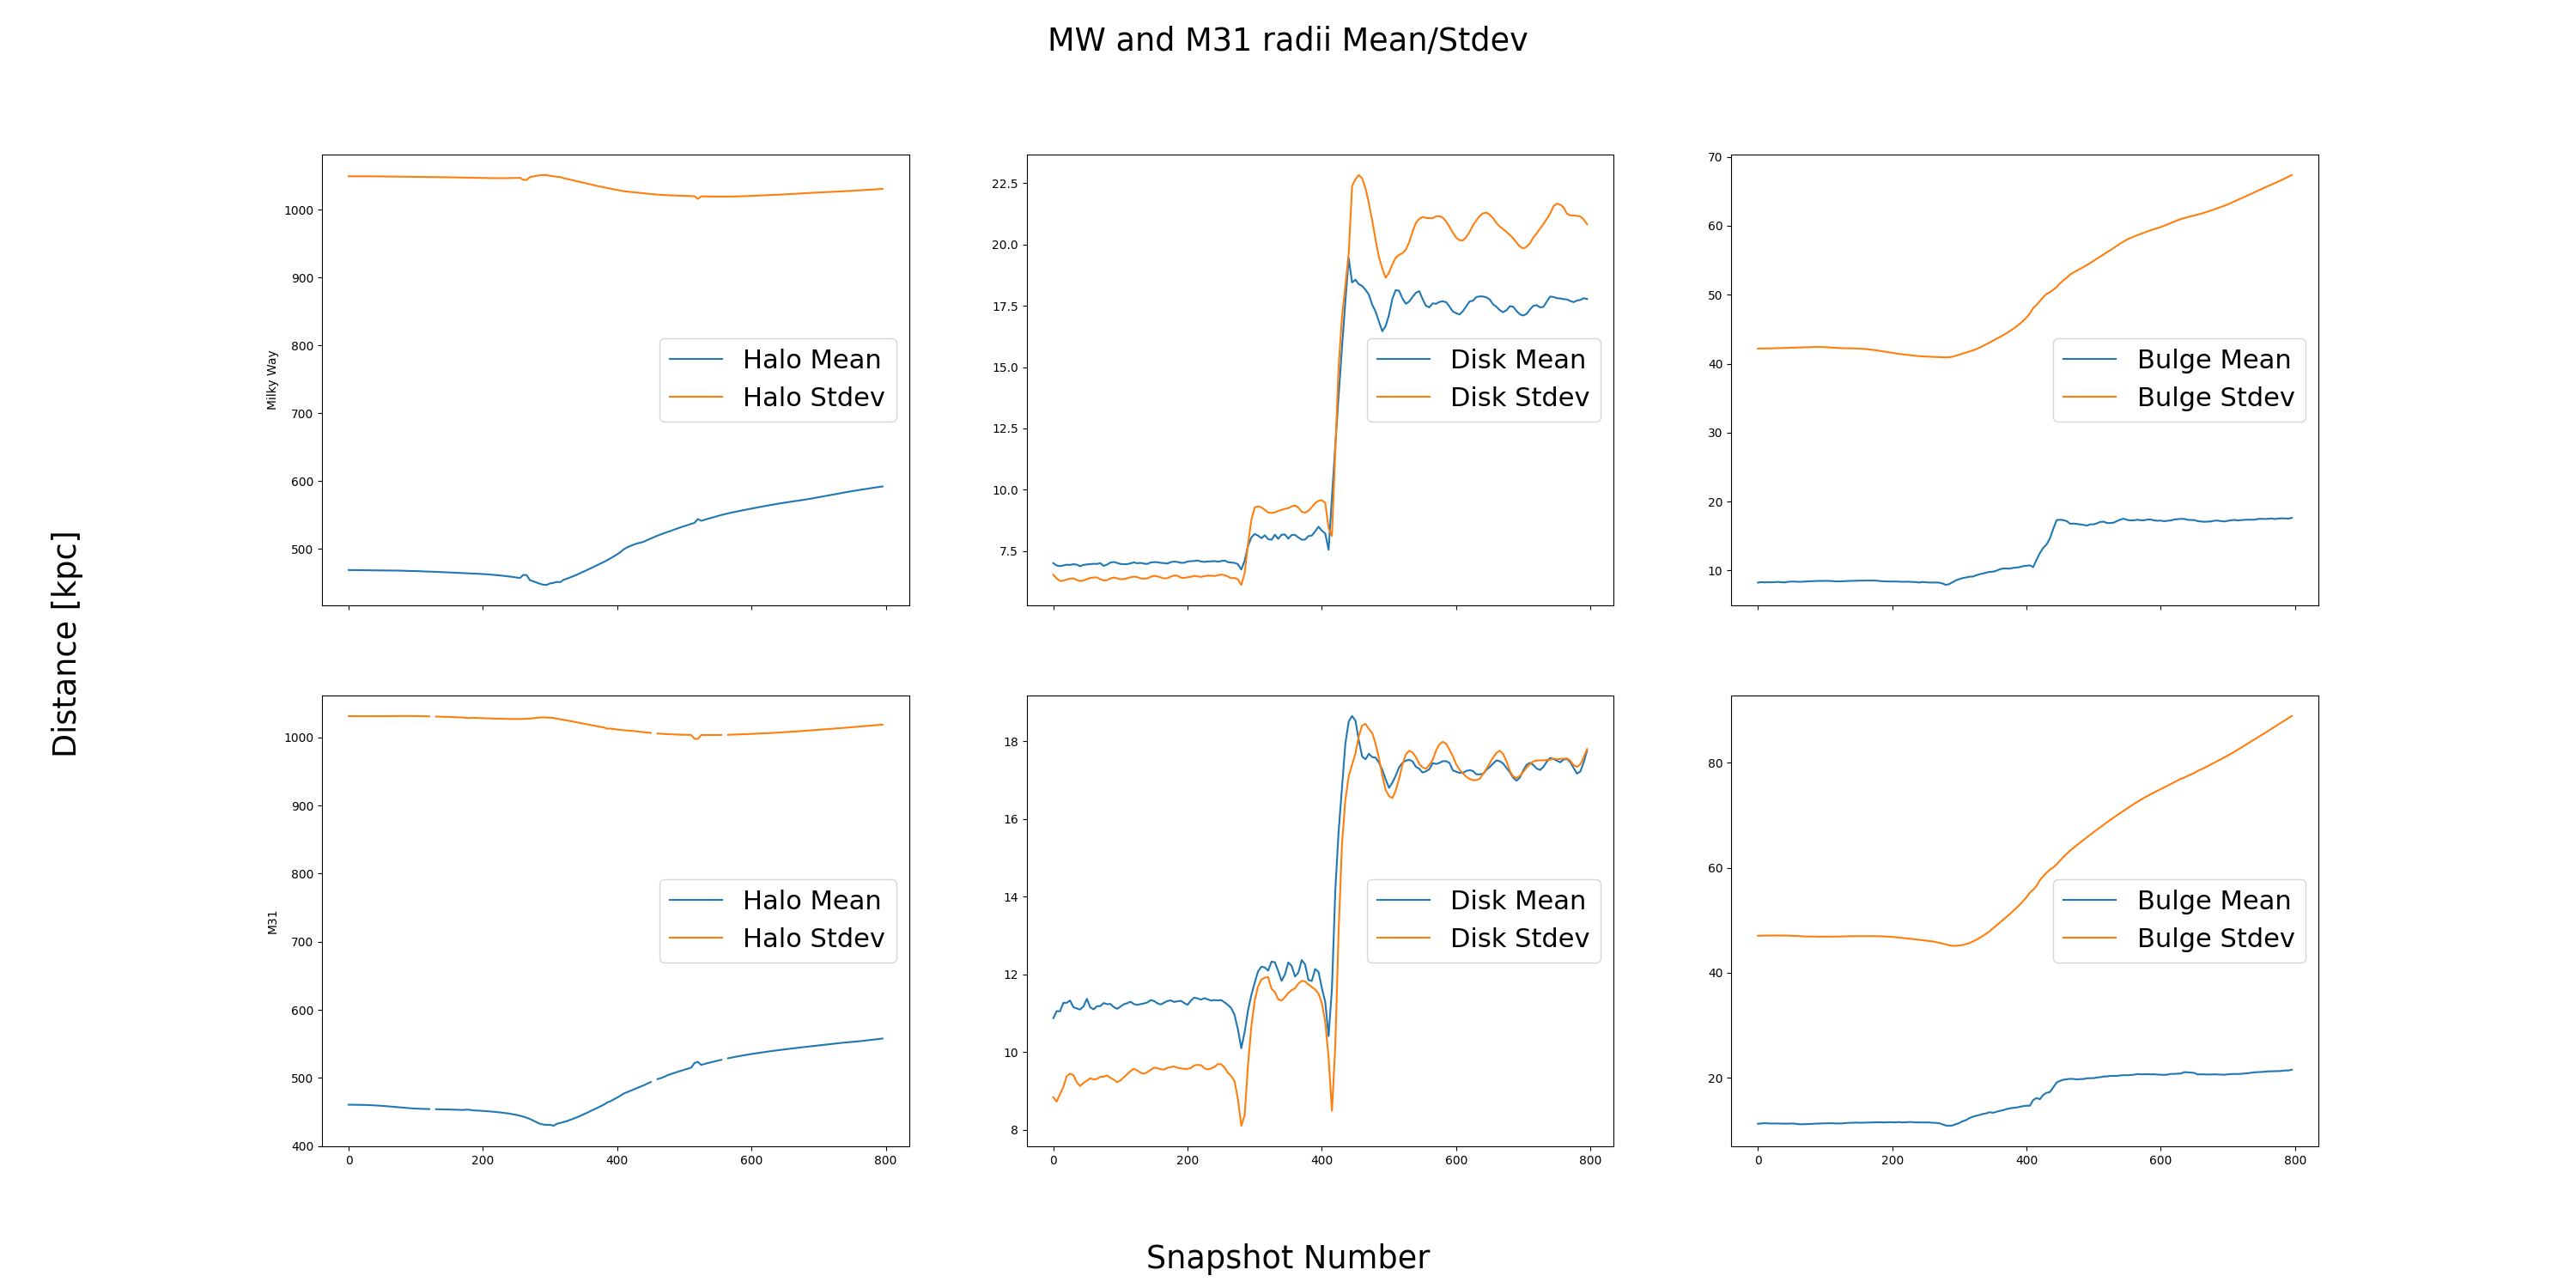
\includegraphics[width = \linewidth]{figures/meanstdev.png}
    \label{fig:meanstdev}
    \caption{The Mean and Standard Deviation of the galactocentric radius for every particle in M31 and the MW. Snapshot number is along the x-axis, and radius (kpc) along the y-axis. We plot all particle types separately to show their different dynamics. This illustrates the disruption of the galaxy during the merger, and the gradual outwards migration of the particles with time as the systems fall together to form an irregular galaxy. Note that while the most dramatic shifts during the merger (Snapshot no. ~300-400) are seen in the Bulge and Halo Particles, once one takes into account the relative size of the perturbation, the Disk Particles are most heavily affected. This implies that, while the Disk is torn apart during the merger, the Bulge and Halo remain mostly intact.}
\end{figure}


\begin{figure}[ht!]
\centering
   \subfloat[\label{genworkflow}]{%
      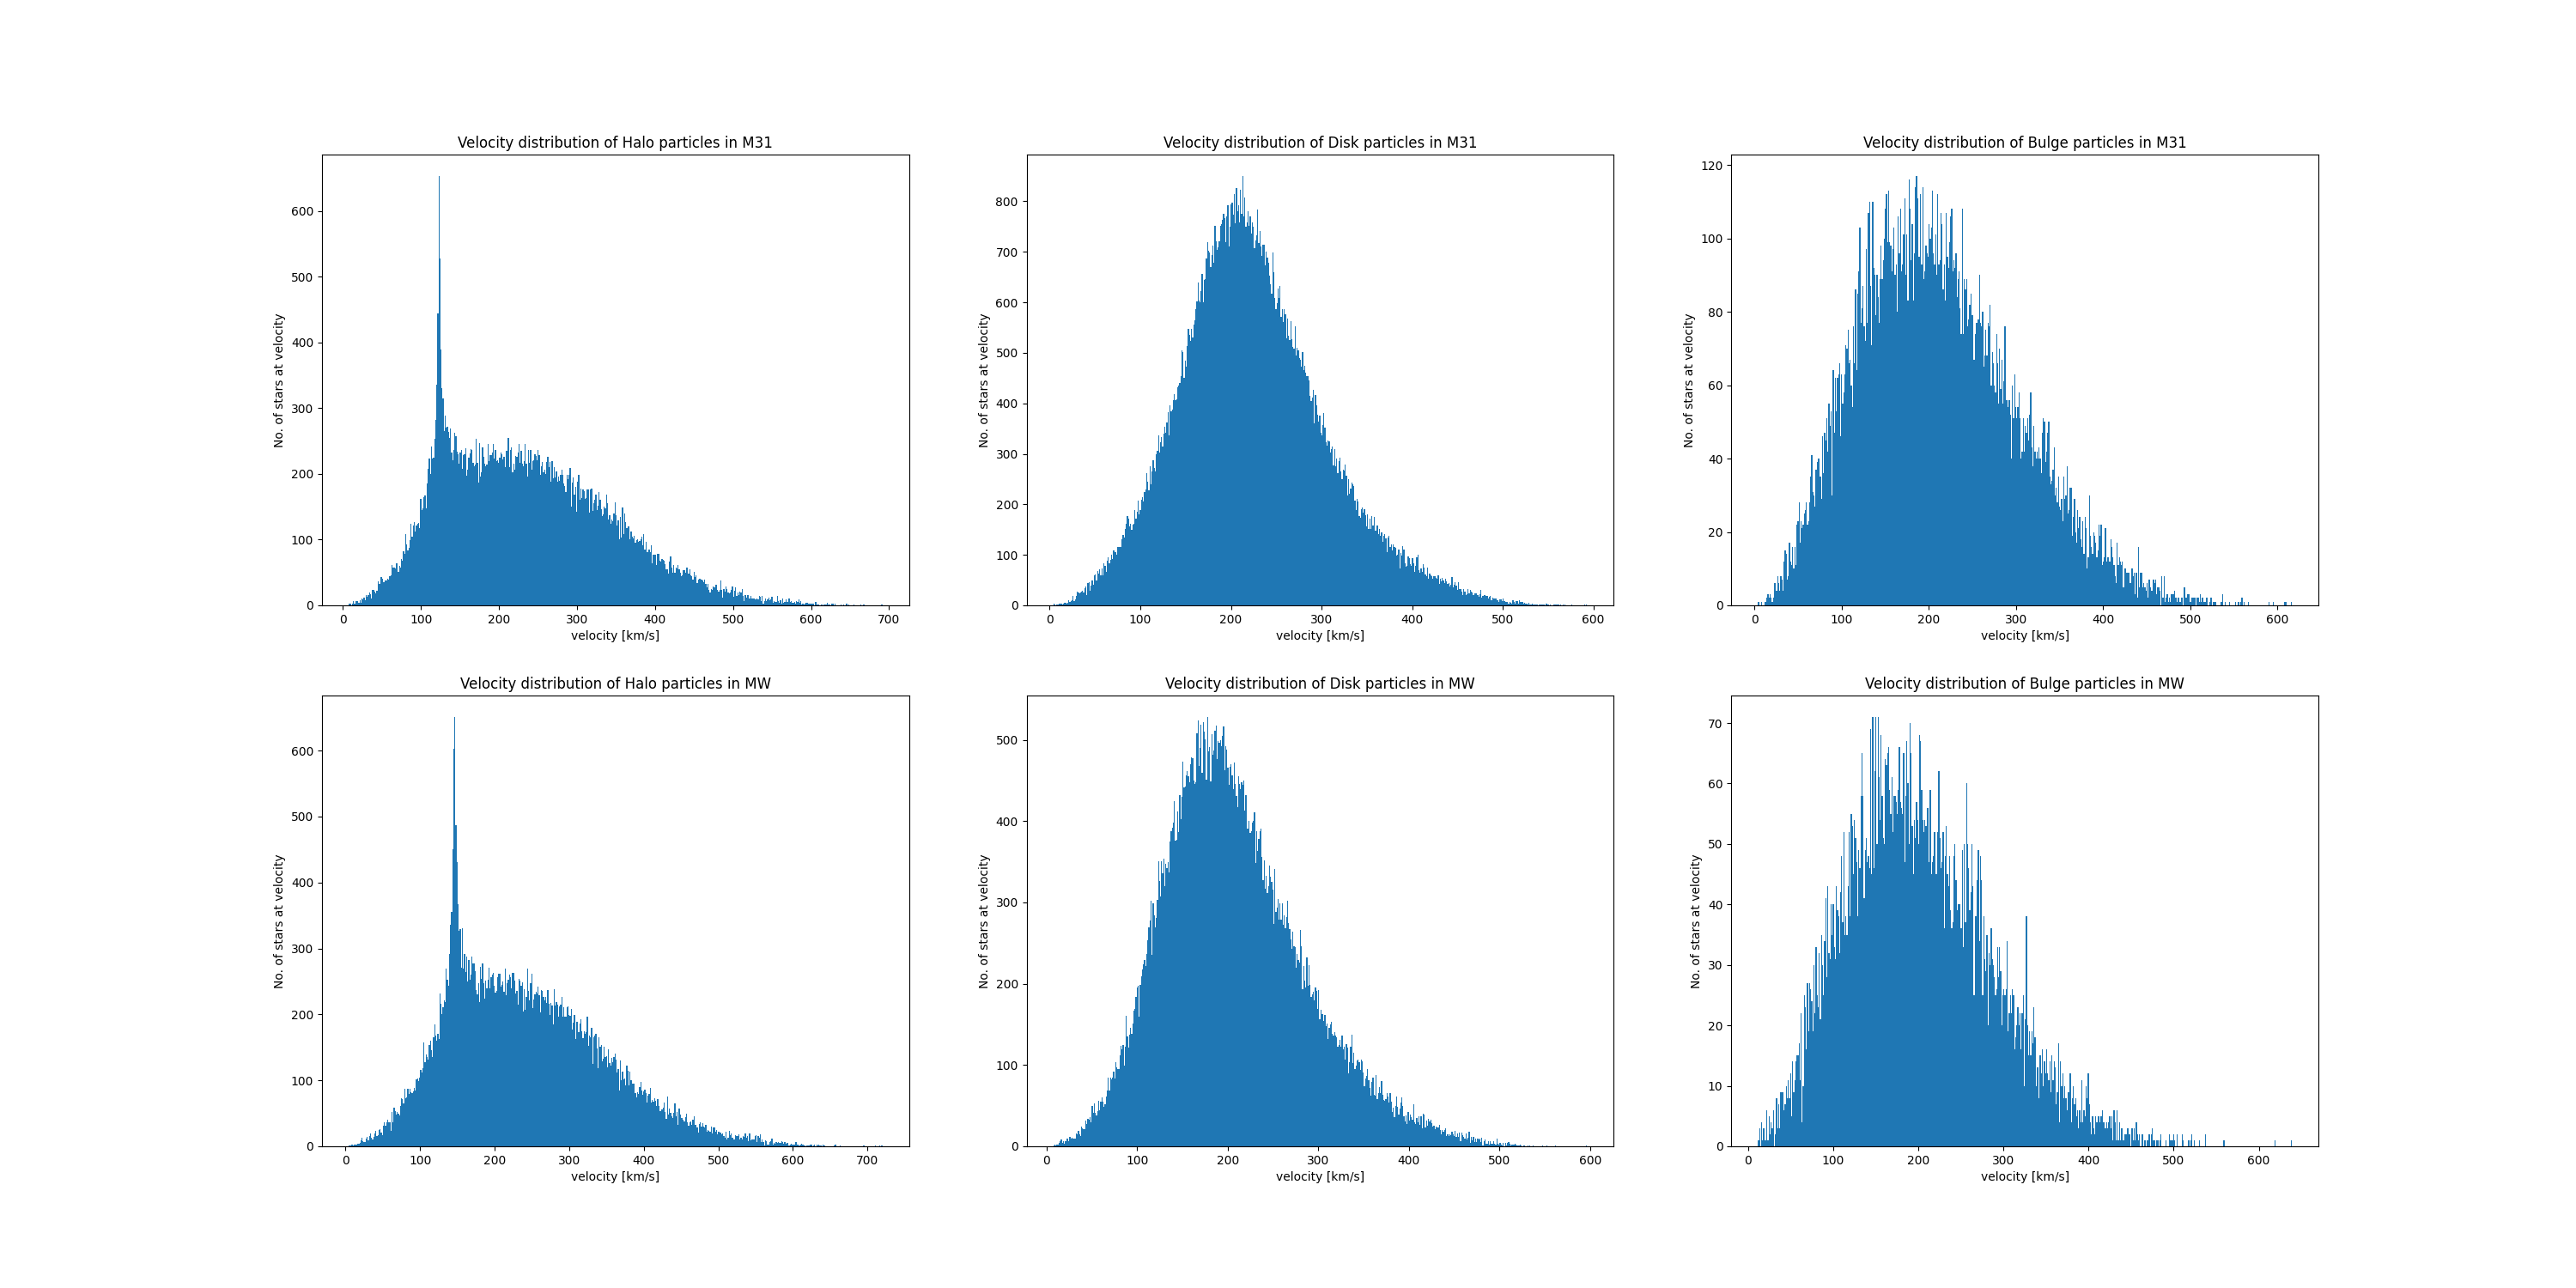
\includegraphics[trim=20 40 50 30,clip, width=0.6\textwidth]{figures/vhist300.png}}
      
   \subfloat[\label{pyramidprocess} ]{%
      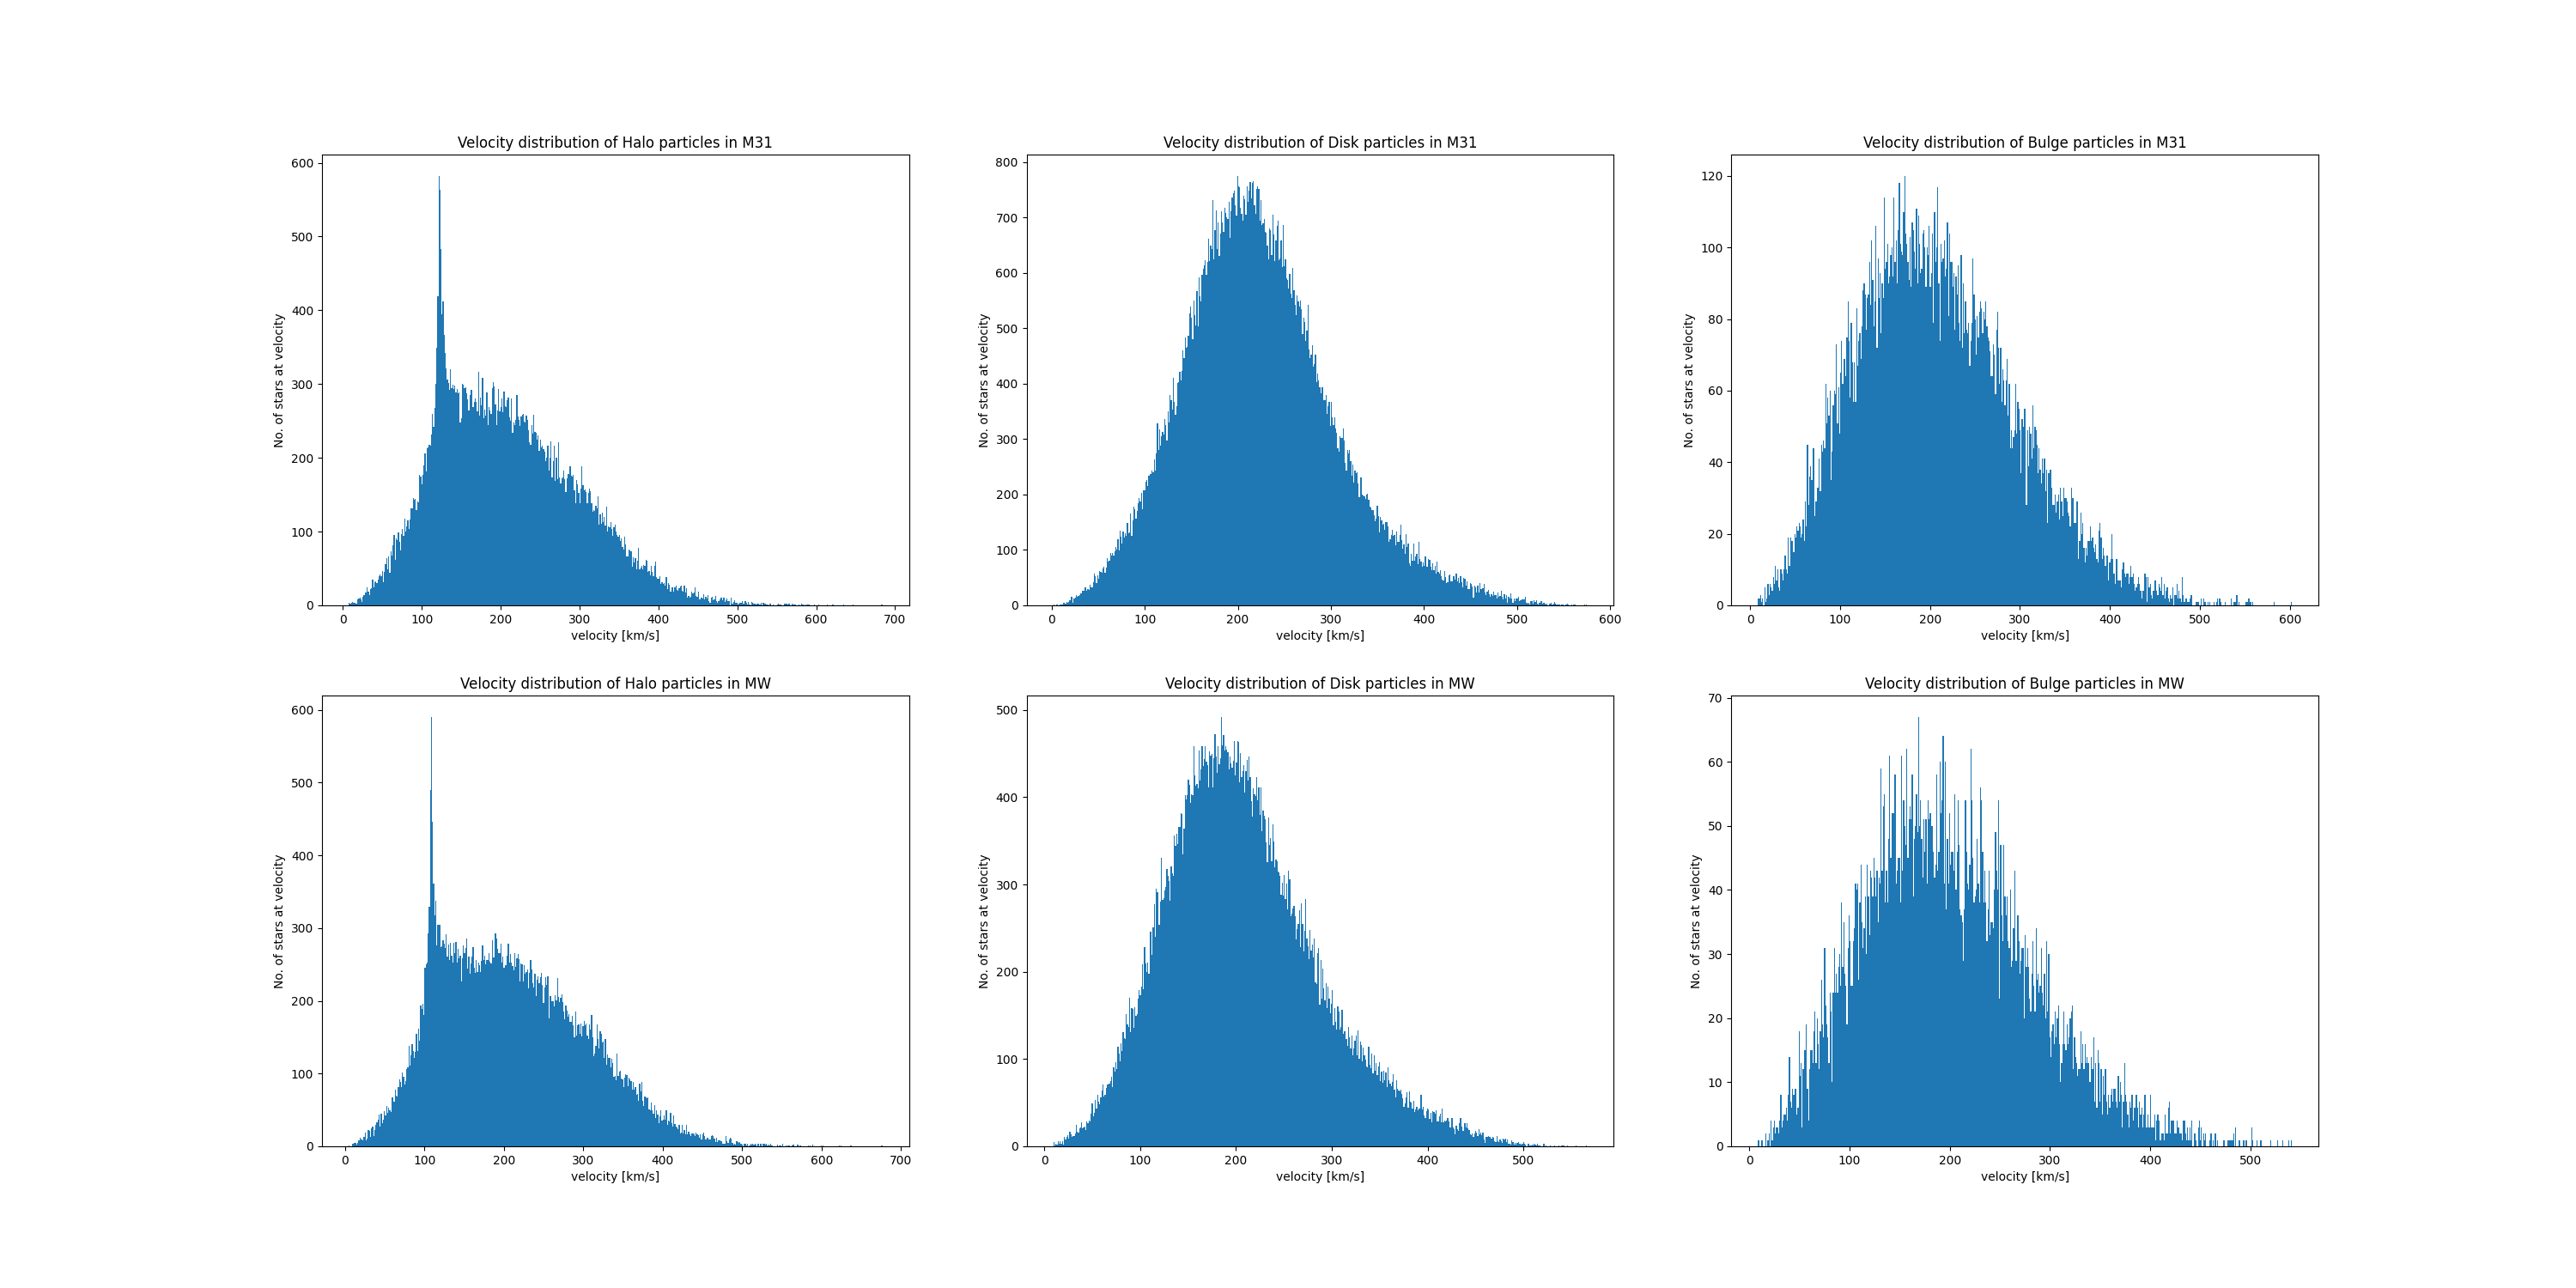
\includegraphics[trim=10 40 10 30,clip, width=0.6\textwidth]{figures/vhist380.png}}
      
   \subfloat[\label{mt-simtask}]{%
      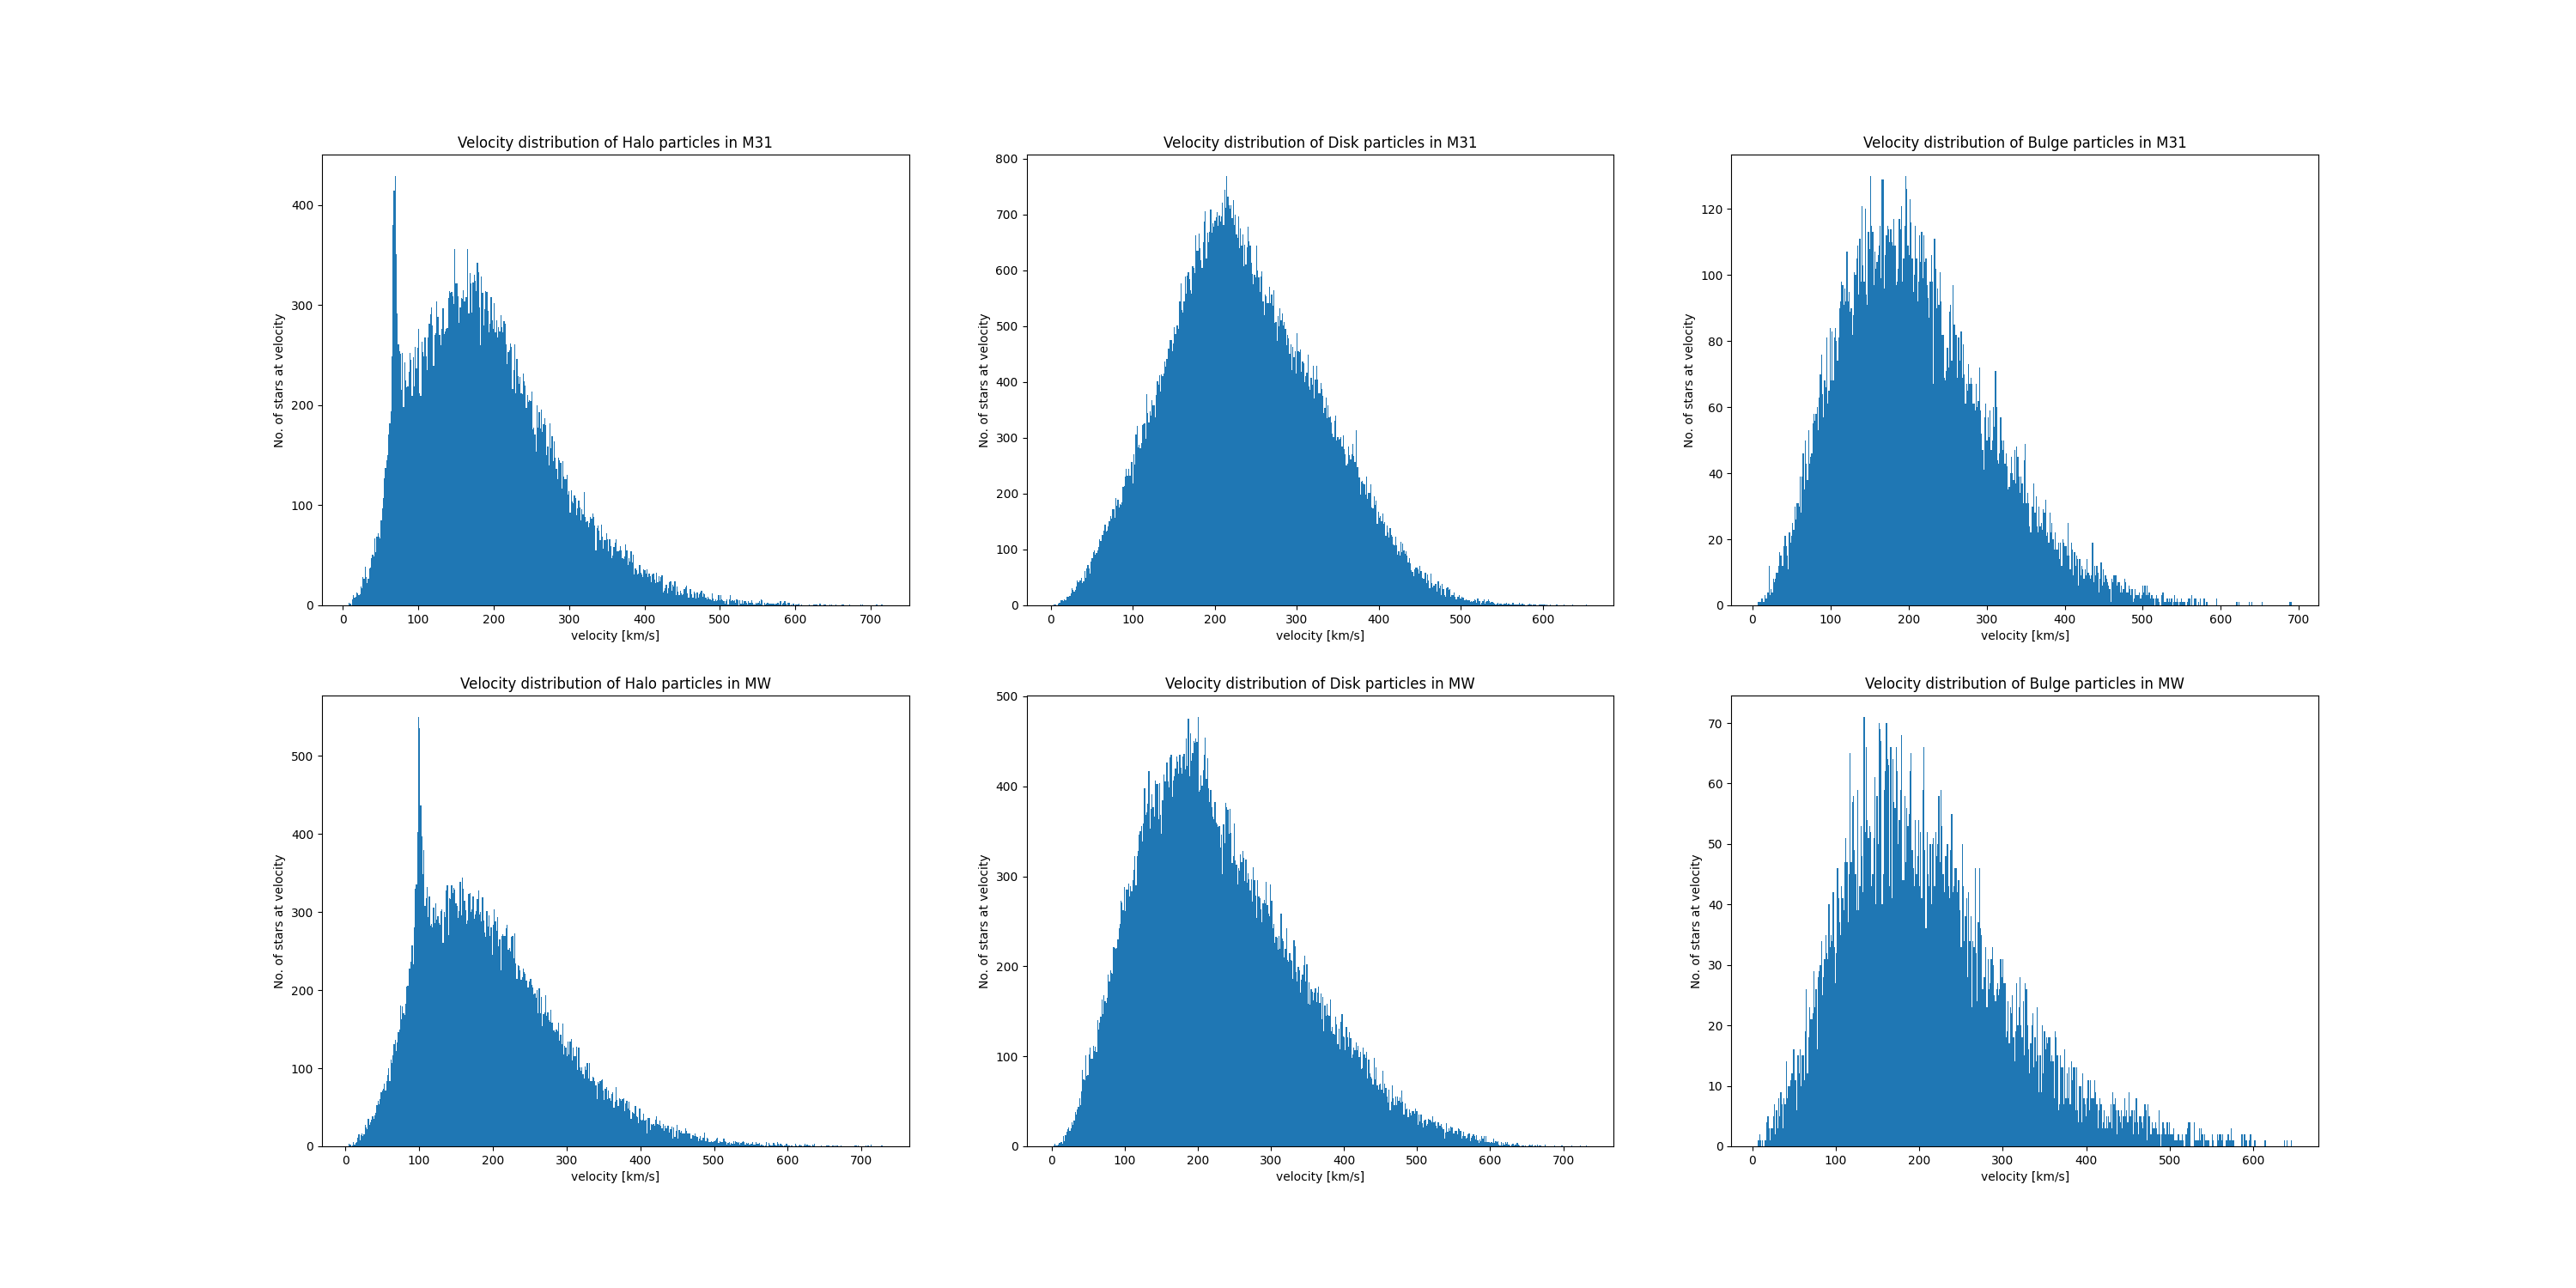
\includegraphics[trim=30 40 30 30,clip, width=0.6\textwidth]{figures/vhist440.png}}\\
      
\caption{\label{fig:vdists} Histograms of velocity distributions (km/s) pre-, during, and post- first close encounter. (a) Snapshot 300; (b) Snapshot 380; (c) Snapshot 440. The different particle types are Halo, Disk, and Bulge, from left to right. The top row shows results for M31, the bottom for M33. The x-axis gives velocities in km/s, while the y-axis gives the number of particles at that velocity. There is not an appreciable difference, unlike the plot of radial displacement, and there are barely any outliers. This demonstrates the awesome power of dynamical friction, the friction caused by the wake as a particle moves through a field of dark matter. Any material that is flung outwards is unable to gain much kinetic energy, and what little it can is quickly lost and the particle ends up falling back inwards.}
\end{figure}

\begin{figure}[ht!]
\centering
   \subfloat[\label{genworkflow}]{%
      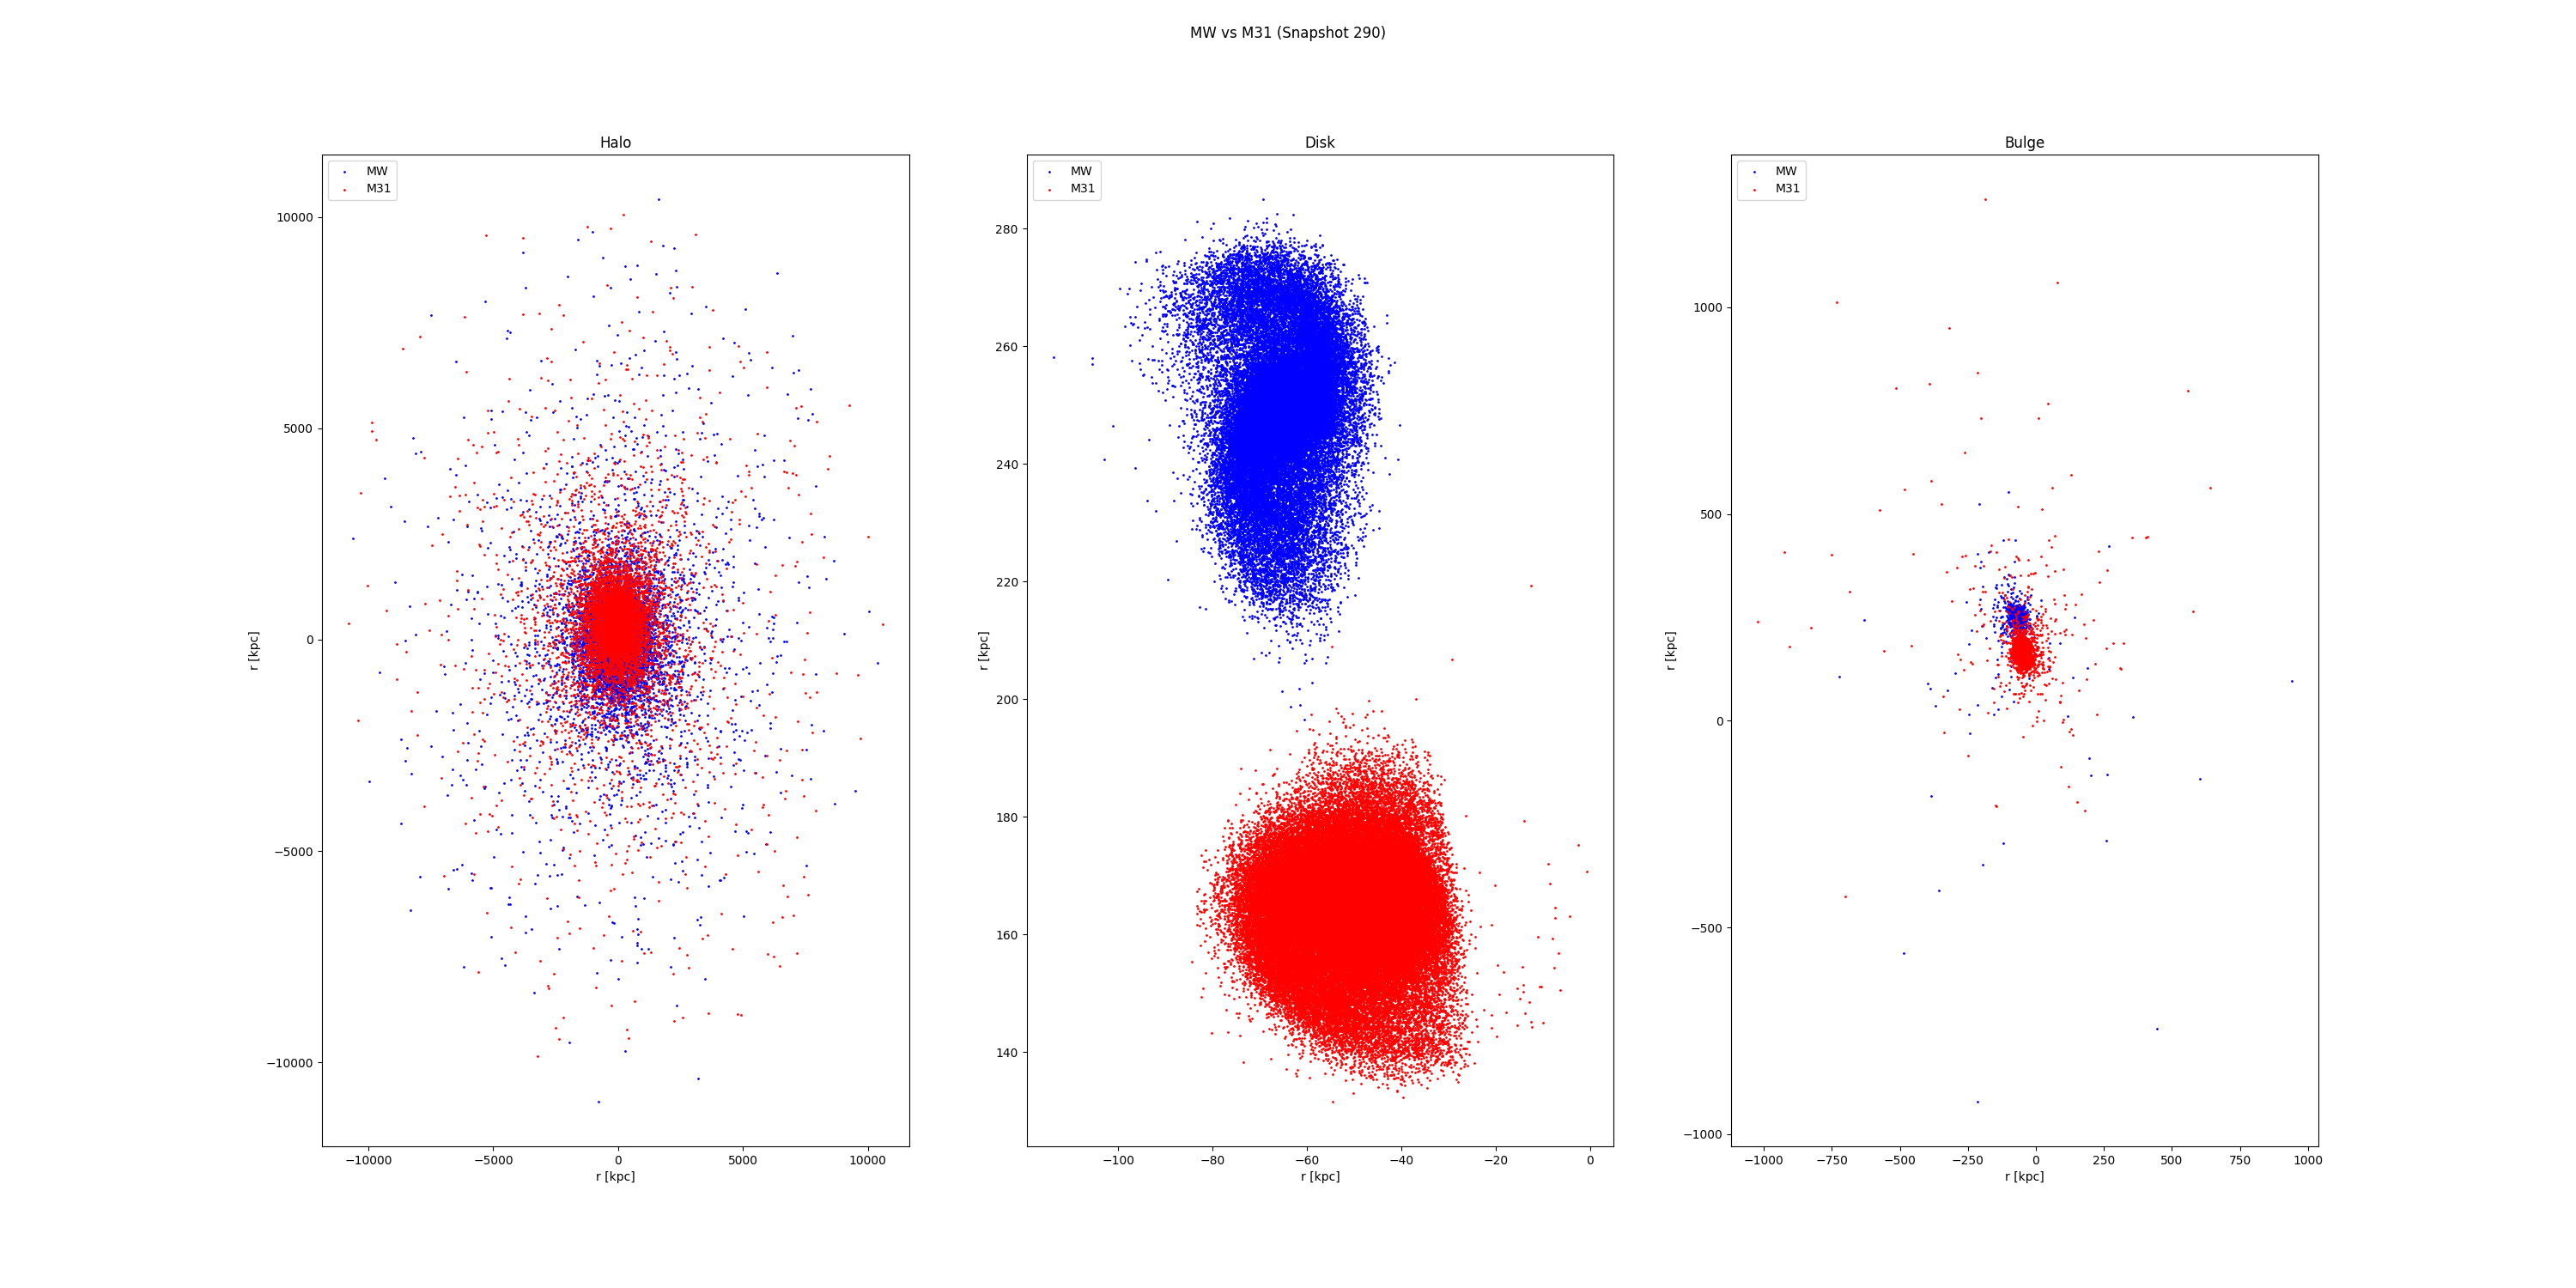
\includegraphics[trim=20 40 50 30,clip, width=0.6\textwidth]{figures/290.png}}
      
   \subfloat[\label{pyramidprocess} ]{%
      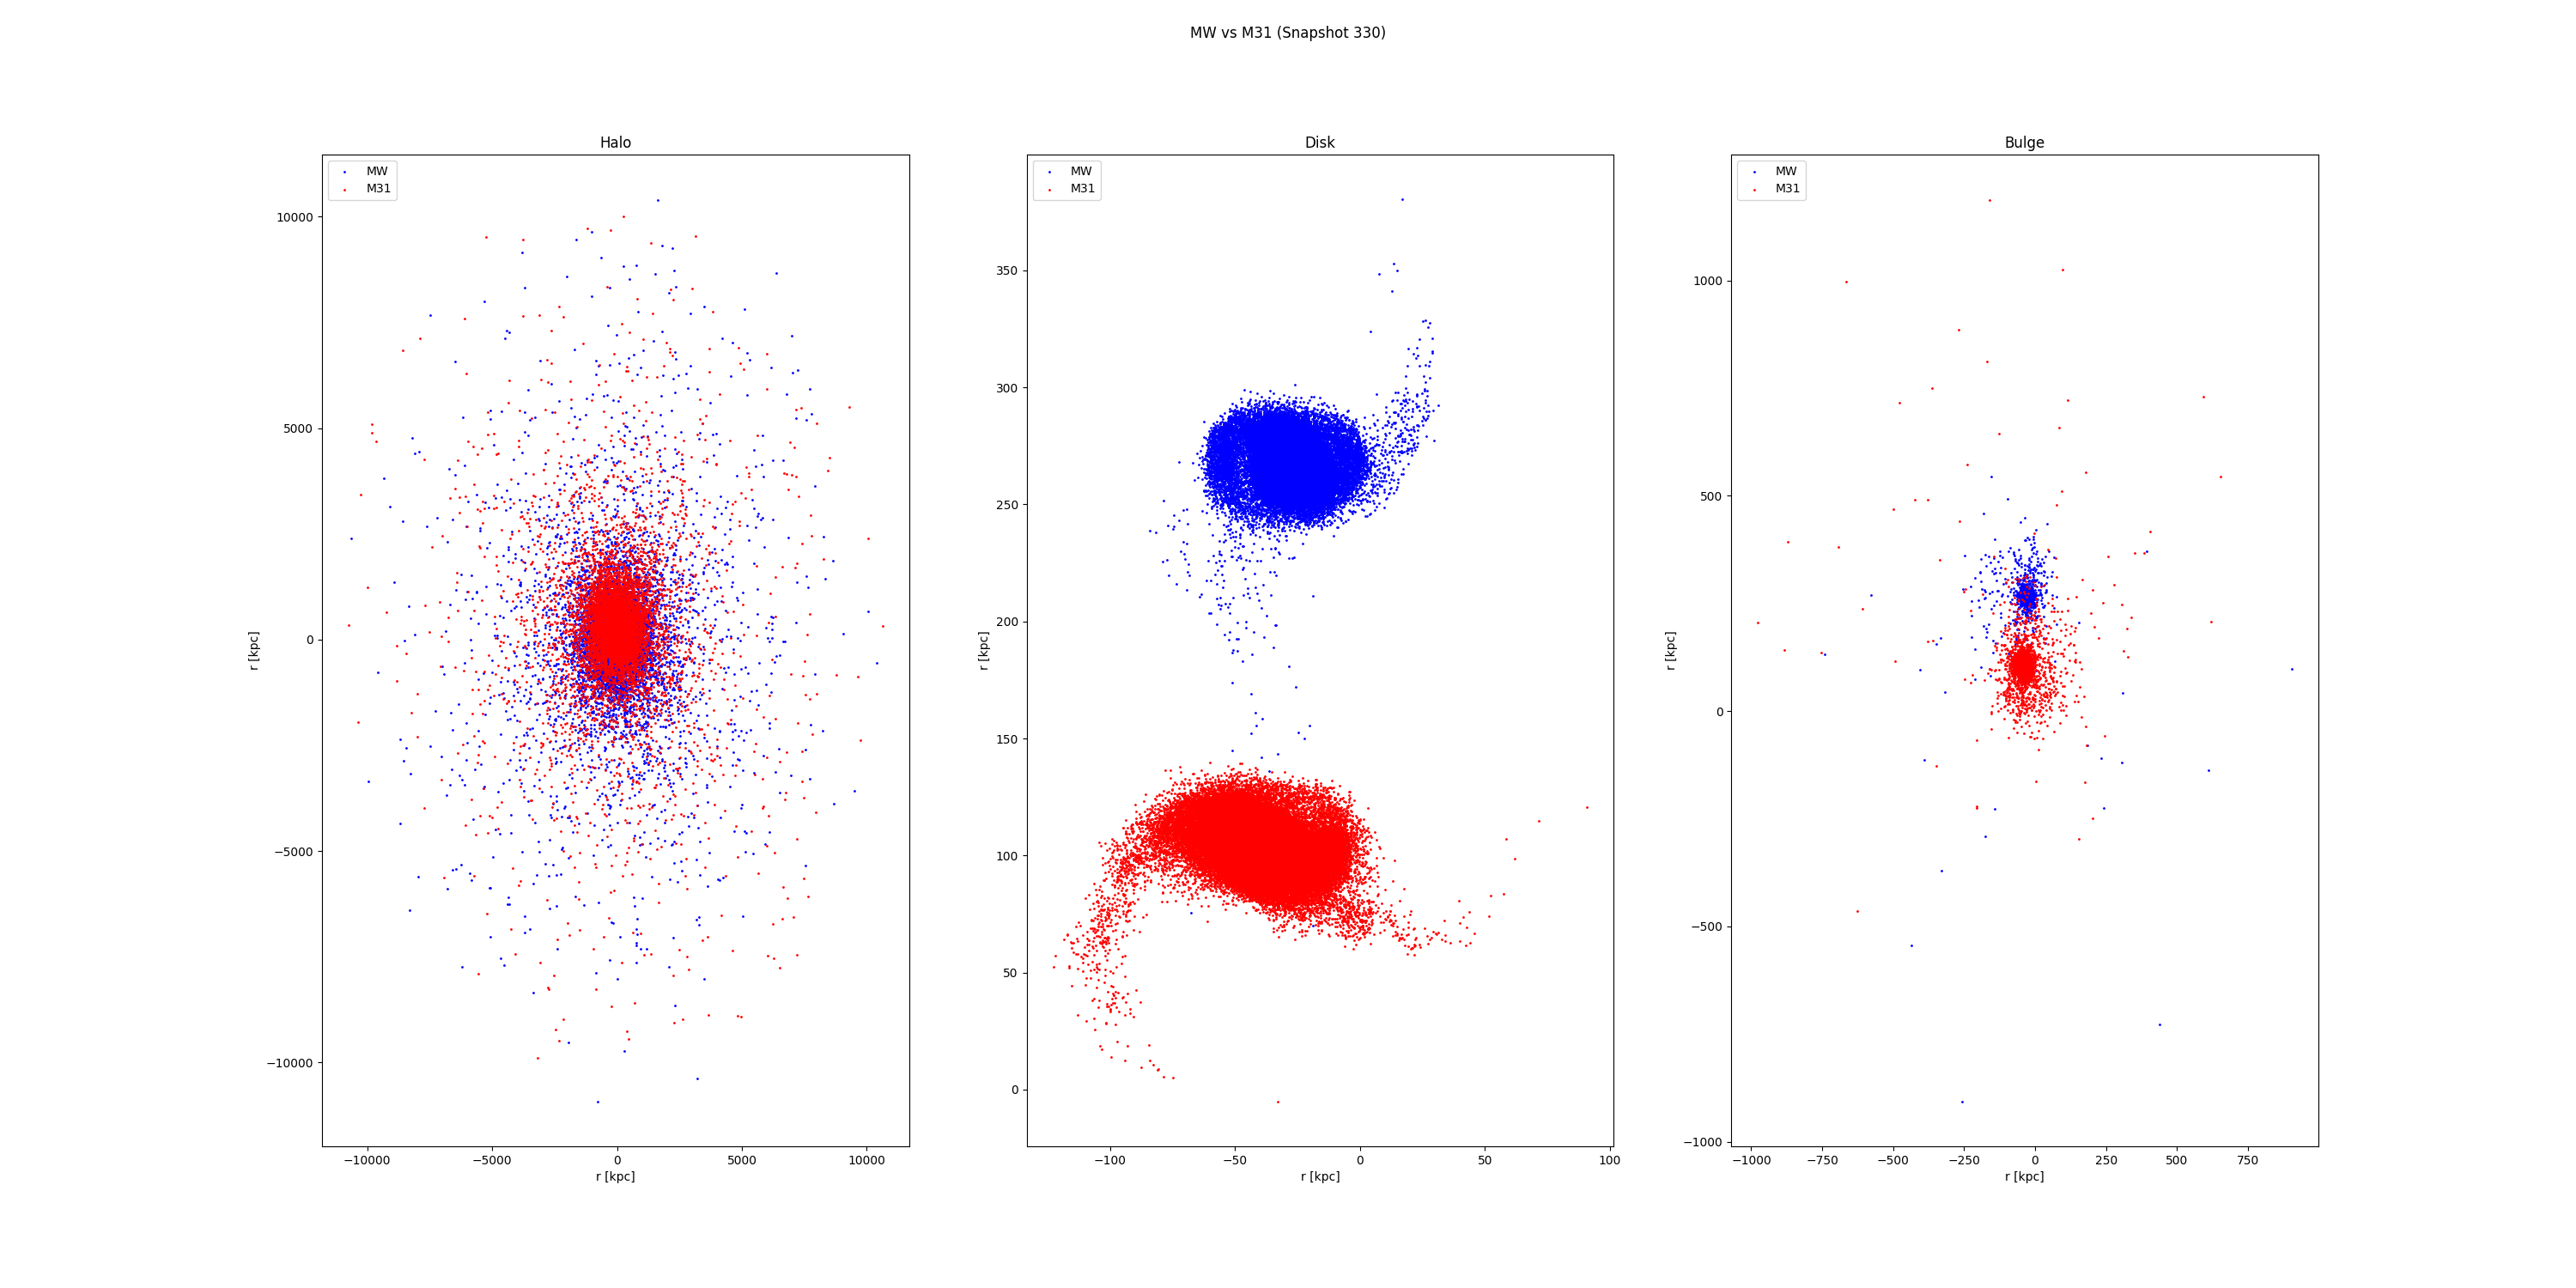
\includegraphics[trim=10 40 10 30,clip, width=0.6\textwidth]{figures/330.png}}
      
\caption{\label{fig:2dproj} A simple 2D projection of the particles of the galaxies during the merger. (a) Snapshot 290; (b) Snapshot 330. The different particle types are Halo, Disk, and Bulge, from left to right. The x- and y-axes give distance in kpc. We note the mass transfer (though it is hard to see, and much better illustrated in the accompanying movie) and the huge displacement of particles from their respective galactic centers.}
\end{figure}

There are four main figures created. The first (Figure \ref{fig:potentialdists}) is a histogram of the Total Energy of particles in each galaxy with respect to (a) its host galaxy and (b) the other galaxy. It can be used to see how the system evolves with time and, importantly, to see if particles can end up gravitationally unbound. The answer, as is evident in the figure, is no. The potentials stay largely the same with time, even for the disk as it is being torn apart, demonstrating the true gravitational power the combined system has. At these energies, no particles will escape.

The second figure gives us an idea of how the system has been disrupted. Figure 4 provides us with the mean and standard deviation of the galactocentric radii of the particles in the system. Though the energies remain largely homogeneous, the displacements are immense, demonstrating just how far out the merger has flung the mass in the galaxies and disrupted their regular rotation.

The third figure (Figure \ref{fig:vdists}) is similar to Figure \ref{fig:potentialdists}. It is a histogram of the velocity distributions (km/s) of all the particles in the galaxy, before, during, and after the merger. Once more, we note that there is little change in the velocities over time, and few outliers. This is a good demonstration of dynamical friction.

The final set of figures (Figure \ref{fig:2dproj}) are a simple 2D projection of each particle type over the course of the merger and the close encounters that precede it. These a good visual check for how badly different parts of the galaxy are affected by the merger.

The movies created of these simulations are available on Github.

\section{Discussion}
Let's look at Figure \ref{fig:potentialdists}. There is very little change over time, even through multiple close encounters. This tells us that the merger, violent though it is, does not appreciably change the velocity of the particles or the displacement from the Center of Mass enough for it to be reflected in the total energy. The potential term is simply too massive.

Further analysis leads us to a somewhat surprising result - particles are never unbound! During our simulation, there is no point at which a particle ends up gravitationally unbound. While at first this seems suspect, it makes more sense in hindsight - during the MW/M31 collision, the only particles significantly kinematically perturbed (as reflected in Figure 4) are the Disk particles. These, too, only escape out to distances of about $20kpc$, leaving the bulk of the mass still bound to the galaxies. What kinetic energy is gained drops off very quickly (see Figure \ref{fig:vdists}) due to the effects of dynamical friction, courtesy of the $\sim 100kpc$ Dark Matter Halos surrounding the system. So, during the actual MW/M31 merger, there will likely be very few stars that manage to escape beyond the gravitational well of the combined system. The best they can do is transfer from one galaxy to another, which brings us neatly on to our next figure.

Figure 4 shows us how disruptive the first close encounter is, and the deformation of the galaxies. Once more, the strongest effect is seen in the disk particles, which go from hovering below 5kpc all the way up to 18kpc, with fluctuations with each subsequent close encounter. The Halo, in the grand scheme of thing, is almost completely unaffected, though that is only because of the immense scale. It fluctuates by almost 50kpc. The bulge's evolution is significantly more damped than the disk's, but is still very violent - the mean radius changes from 40 to over 60kpc, and it seems to keep rising. This might be indicative of the combined system tending towards a more spherically symmetric shape towards the end of the merger.

Let's look more closely at the merger itself. Figure \ref{fig:2dproj}
shows us the mass transfer between our galaxies, and it effectively demonstrates the mass transfer and immense displacement of particles. The mass transferred from M31 (red) to the MW (blue) largely ends up close to the galactic centre, which aligns with our expectation. However, it also shows that the particles which are flung out do not become gravitationally unbound, as eventually they end up falling back into the centre. This is somewhat reflected in Figure 4, which implies that particles aren't being gravitationally unbound, instead they are finding a new equilibrium at which they can rotate in the now-combined system.


\section{Conclusion}

Our aim was to study the evolution of the Milky Way/M31 galactic merger. Specifically, the nature of the mass transfer during the merger and the evolution of the system with time. We have tracked different variables in the pursuit of our results, e.g. the mean galactocentric radius with time, the Energy over time, and have visualized the merger itself to confirm mass transfer between the systems.

We have found that mass transferred between the systems is most likely to end up near the galactic centre, where the bulk of the mass of the galaxy is concentrated. This is a result that agrees with our hypothesis, and means that most mass transfer between galaxies exchanges particles into the disk.

We have also found that it is exceedingly difficult for galactic particles to become gravitationally unbound from the system. The vast masses involved couple with the dynamical friction effects of dark matter to ensure that particles cannot easily escape. Indeed, all particles flung out from the disk end up slowly drifting back inwards. This disagrees with our initial hypothesis, but in retrospect, the presumption was a little naive. 


There are many ways the code could be improved, e.g. plotting the distance of particles from the other galaxy's galactic center over time, or even better visualization of the results. We could also run this data over more timesteps (all data was currently run with snapshot increments of 5 at minimum), or with the HighRes data instead of the LowRes.

\section{Acknowledgements}
I would like to thank Dr. Gurtina Besla and Hayden Foote for their invaluable input and help on this project.

This research made use of NumPy \citep{harris2020array}. This research made use of matplotlib, a Python library for publication quality graphics \citep{Hunter:2007}. This research made use of Astropy, a community-developed core Python package for Astronomy \citep{2018AJ....156..123A, 2013A&A...558A..33A}. This work made use of the IPython package \citep{PER-GRA:2007}.

\bibliography{sample631}{}
\bibliographystyle{aasjournal}

\end{document}